\newpage
\chapter[Case study]{\thechapter. Case study}
\section{Overview}
The design architecture used in AUTOSAR represents the layered pattern\footnote{Automobil-Elektornik - January 2007 - S.28} using a component-based approach. One of the key benefits of this kind of architecture, which is applied extensively in software development, are the well-defined interfaces and strong dependency management.\newline
As mention in 1.1 this case study will impact only the modeling of the memory stack as shown in Figure 2.1.
\begin{center}
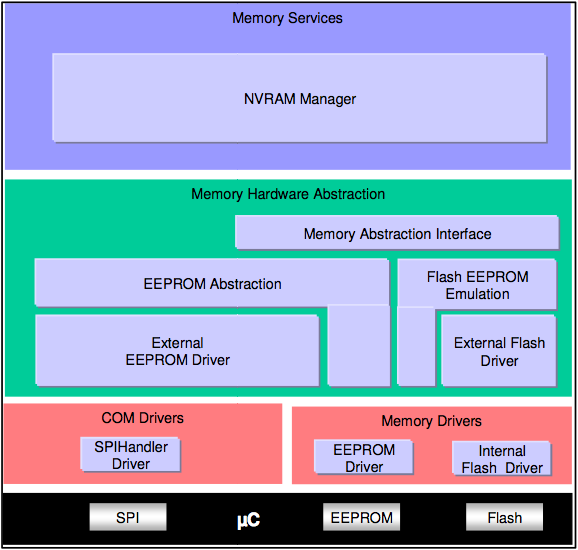
\includegraphics[scale=0.55]{Images/Figure2_1.png}\\
Figure 2.1 - Memory stack
\end{center}
\newpage
%Variable for functional requirements
\newcommand{\FR}{BSW}

\section{Requirements}
\subsection{Overview}Each module specific section contains a short functional description of the software module.Each module specific section contains a short functional description of the software module.

\subsection{NVRAM-Manager}
The \mbox{NVRAM} manager, as specified in [AUTOSAR$\_$SRS$\_$MemoryServeices.pdf], is highly scalable and hardware independent, thus making it usable in all domains of an automotive system. Providing service to manage the storage of data in all kinds of non-volatile memory and reliability mechanisms.

\subsubsection{Acronyms and abbreviations}
{\bf Basic Storage Object} - The smallest entity of a NVRAM Block.\newline
\newline 
{\bf NVRAM Block} - The entire structure, that administrate and stores a block of NV data.\newline
\newline
{\bf NV data} -  The stored data in the non-volatile memory.\newline
\newline
{\bf Block Management Type} - Type of the NVRAM block. It depends on the individual composition of a NVRAM block in chunks of different mandatory or optional Basic Storage Objects and the subsequent handling of this NVRAM block.\newline
\newline
{\bf RAM Block} - A Basic Storage Object, that represents a part of a NVRAM block in RAM.\newline
\newline
{\bf ROM Block} - A Basic Storage Object that represents an optional part of a NVRAM block in ROM.\newline
\newline
{\bf NV Block} -  A Basic Storage Object that represents a mandatory part of a NVRAM block in NV memory.\newline
\newline
{\bf Administrative Block} - A Basic Storage Object that resides in RAM. It contains any RAM data, that are necessary to manage the NVRAM block.

\subsubsection{Functional requirements}

\subsubsection{Configuration}
{\bf [\FR041]} - Each application shall be enabled to declare and allocate the memory requirements at configuration time.\newline
\newline
{\bf [\FR08534]} - Two classes of RAM data blocks shall provide the service for data exchange between the NVRAM-Manager and SW-Components.\newline
\newline
{\bf [\FR08528]} - The basic storage of data and ROM configurable ROM defaults shall be provide from the native \mbox{NVRAM} block.\newline
\newline
{\bf [\FR08529]} - Data shall be provide in case of inconsistencies by the redundant  \mbox{NVRAM} block, which is transparent to application.\newline
\newline
{\bf [\FR08531]} - To allow runtime selection of different datasets in \mbox{ROM$\backslash$`NVRAM}, a dataset  \mbox{NVRAM} shall be configurable to include default values.\newline
\newline
{\bf [\FR08543]} - The priority of each NVRAM block shall be statically configurable in different levels.\newline\newline
{\bf [\FR08009]} - For each \mbox{NVRAM} block there shall be a static configuration of a default write protection, which shall be done by the \mbox{NVRAM-Manager}.\newline
\newline
{\bf [\FR08549]} - After a software update,the \mbox{NVRAM}manager shall provide functionality to automatically initialize RAM data blocks with ROM defaults.\newline
\newline
{\bf [\FR125]} - For each block a notification shall be configurable, which will initiated after a completion of a read/write job.\newline
\newline
{\bf [\FR135]} - There shall be a configuration ID, that could be either statically assigned to the configuration or it can be calculated. This ID would be stored separately and should be used to determine the validity of the NVRAM contents.\newline
\newline
{\bf [\FR08000]} - The NVRAM manager shall be able to access multiple non-volatile memory devices, which can be of different type.\newline
\newline
{\bf [\FR08001]} - The NVRAM manager shall be check each block for consistency.\newline
\newline
{\bf [\FR08538]} - One kann statically configurate which blocks are going to be automatically loaded at startup of the NVRAM manager.\newline
\newline
{\bf [\FR08546]} - For each NVRAM block there shall be a configurable option to enforce meachnisms increasing integrity of \mbox{RAM} data.\newline
\newline
\subsubsection{Initialization}
{\bf [\FR08533]} - The \mbox{NVRAM} manager provides a service to check and load those \mbox{NVRAM blocks}, that are configured to have a permanent \mbox{RAM} data block.\newline
\newline
\subsubsection{Normal Operation}
{\bf [\FR176]} - The \mbox{NVRAM} manager could only access the non-volatile memory.\newline
\newline
{\bf [\FR027]} - The \mbox{NVRAM} manager provides an implicit way of accessing blocks in the \mbox{NVRAM} and in the \mbox{RAM}.\newline
\newline
{\bf [\FR08014]} - The \mbox{RAM} block would be defined as not continuos in the global \mbox{RAM} area.\newline
\newline
{\bf [\FR013]} - The \mbox{NVRAM} manager would be able to handle concurrent accesses to  \mbox{NVRAM} memory.\newline
\newline
{\bf [\FR016]} - The \mbox{NVRAM} manager would be able to read out data associated with an  \mbox{NVRAM} block from the non-volatile memory.\newline
\newline
{\bf [\FR017]} - The \mbox{NVRAM} manager would be able to store data associated with a \mbox{NVRAM} block in the non-volatile memory.\newline
\newline
{\bf [\FR08541]} - The \mbox{NVRAM} manager would accept and process any write request.\newline
\newline
{\bf [\FR018]} - The \mbox{NVRAM} manager would be able to restore a\mbox{NVRAM} block's associated data from \mbox{RAM} defaults.\newline
\newline
{\bf [\FR08547]} - The \mbox{NVRAM} manager is able to distinguish between explicitly invalidated and inconsistent data.\newline
\newline
{\bf [\FR08548]} - The \mbox{NVRAM} manager is able to request the default data from the application, if there is no \mbox{ROM} block available at configuration time.\newline
\newline
{\bf [\FR08550]} - The \mbox{NVRAM} manager is able to mark \mbox{RAM} data blocks as modified or unmodified. This service is configurable.\newline
\newline
{\bf [\FR08545]} - The \mbox{NVRAM} manager is able to mark the parmanent \mbox{RAM} data block of a \mbox{NVRAM} block valid. This configurable service could also update integrity information, if configured.\newline
\newline
{\bf [\FR08011]} - The \mbox{NVRAM} manager is able to invalidate an block of data in the non-volatile memory. This service is also configurable.\newline
\newline
{\bf [\FR08544]} - The \mbox{NVRAM} manager is able to erase the NV block or blocks associated with a \mbox{NVRAM} block, if configured.\newline
\newline
{\bf [\FR08007]} - The \mbox{NVRAM} manager  could associate a dataset number to the corresponding \mbox{RAM} block.\newline
\newline
{\bf [\FR08542]} - The \mbox{NVRAM} manager provides a scheduling service for jobs. The highest priority job is to be processed first and if there is a job with the same priority level this shall be ececuted in \mbox{FIFO} order.\newline
\newline
{\bf [\FR020]} - The \mbox{NVRAM} manager is able to read out the status of read and write oprations.\newline
\newline
{\bf [\FR127]} - The \mbox{NVRAM} manager is able to enable and disable a write protection for each \mbox{NVRAM} block individually.\newline
\newline
{\bf [\FR030]} - The \mbox{NVRAM} manager is able to check for consistency and integrity of data saved in \mbox{NVRAM} during operation even in case of asynchronous reset or power loss.\newline
\newline
{\bf [\FR034]} - The \mbox{NVRAM} manager write accesses is concurrently executed to normal operation of the \mbox{ECU}.\newline

\subsubsection{Shutdown Operation}
{\bf [\FR08535]} - The \mbox{NVRAM} manager triggers update of integrity information and saving of permanent \mbox{RAM} data blocks to \mbox{NV} memory.\newline
\newline
{\bf [\FR08540]} - The \mbox{NVRAM} manager is to abort a \mbox{ECU} shutdown if a an \mbox{ECU} condition is detected.\newline
\subsubsection{Fault Operation}
{\bf [\FR038]} - The \mbox{NVRAM} manager is not going to report healable or recoverable errors to other software components.\newline
\newline
{\bf [\FR0129]} - If data corruption is detected and valid data can be derived, this is going to be done by the \mbox{NVRAM} manager.\newline
\newline
{\bf [\FR08010]} - If it is not possible for the \mbox{NVRAM} manager read data from \mbox{NV} into \mbox{RAM}, then it will copy the \mbox{ROM} default data to the data area of the corresponding \mbox{RAM} block.\newline
\newline
{\bf [\FR08015]} - After \mbox{ECU} reprogramming some of the \mbox{NV} blocks in the \mbox{NVRAM} are not going to be erased nor be replaced with the default \mbox{ROM} data after the first initialization.\newline
\subsubsection{Non-Functional Requirements}
\subsubsection{Hardware independence}
{\bf [\FR011]} - The \mbox{NVRAM} manager is going to access the underlying memory hardware via interfaces. Thus abstracting the memory hardware.

\subsubsection{Usability}
{\bf [\FR0130]} - The \mbox{NVRAM} manager is providing information in \mbox{MAP} file format how many resources of \mbox{RAM},\mbox{ROM} and \mbox{NVRAM} are being used.
\newpage

%Section Internal Flash Driver
\subsection{Internal Flash Driver}
This driver, as specified in  [AUTOSAR$\_$SRS$\_$Flash$\_$Driver.pdf], provides the ability to initialize, read, write and erase the internal Flash memory. The Flash driver has a built-in possibility to load the flash access code to \mbox{RAM} and execute the write or erase operations from there, if required.\newline
The flash driver is only to be used by the Flash \mbox{EEPROM} emulation module for writing data, if the ECU is in application mode.
\subsubsection{Acronyms and abbreviations}
Such acronyms and abbreviations, that have a local scope do not appear in this section of the document, but in the local glossary.
\subsubsection{Functional requirements}
\subsubsection{Configuration}
{\bf [\FR12132]} - The \mbox{Flash} driver is to be statically configurable.\newline
\newline
{\bf [\FR12133]} - The \mbox{Flash} shall publish diverse properties like: size in bytes, base address, physical memory segmentation and etc.

\subsubsection{Normal Operation}
{\bf [\FR12134]} - With its asynchronous read function can the flash drive a certain data block read, starting at the requested flash address from the internal flash memory with the passed length.\newline
\newline
{\bf [\FR12135]} - With its asynchronous write function can the flash drive a certain data block write, starting at the requested flash address from the internal flash memory with the passed length. If the requested flash address is unaligned to the physical memory segment, this request shall be rejected with an error code.\newline
\newline
{\bf [\FR12136]} - With its asynchronous erase function can the flash drive a certain segments erase, starting at the requested flash address from the internal flash memory with the passed length. If the requested flash address is unaligned to the physical memory segment, this request shall be rejected with an error code.\newline
\newline
{\bf [\FR12137]} - With the synchronous cancel function can the flash driver stop any currently processed job.\newline
\newline
{\bf [\FR12138]} - The flash driver is able to return the job processing status using. It process is a synchronous function.\newline
\newline
{\bf [\FR12141]} - With the processing of writing the flash drive verifies, if statically configured, the written data by reading back from flash and comparing with the source data. If there are differences, those are going to be notified as errors. \newline
\newline
{\bf [\FR12143]} - The flash drive is able to complete only one job (erase or write) at time. If there is a new job request during an other job, the request will be rejected and handled as error. This detection is statically to be configured.\newline
\newline
{\bf [\FR12144]} - All processing jobs are nested in one processing job. Thus can the flash driver set the status variable.\newline
\newline
{\bf [\FR12158]} - A verification is needed to check if the addressed memory area is being erased, before the flash driver could write data to falsh memory.If this verification is falls, the process would be aborted with an error notification. This feature is to be statically configured.\newline
\newline
{\bf [\FR12159]} - The write and erase functions are providing with a service to check if the address parameters are within the calid configured address borders. If those are beyond the allowed borders, the process will be rejected with a error code.\newline
\newline
{\bf [\FR12160]} - If statically configured, the flash drive is going to check after an erase job, if the addressed block has been erased completely.\newline
\newline
{\bf [\FR12193]} - If an erase or write job is initiated, the flash drive loads the code needed to accesses the flash hardware to \mbox{RAM}. This feature is to be statically configured.\newline
\newline
{\bf [\FR12194]} - To keep the runtime as short as possible, the flash drive executes the code that accesses the flash hardware from \mbox{RAM}. This is only applicable if the code has been loaded to \mbox{RAM}.\newline
\newline
{\bf [\FR13300]} - If statically configured, the flash drive will remove the accesses code from \mbox{RAM} after the erase or write job is been finished or canceled. This is only then necessary if the flash driver has loaded that code to \mbox{RAM} during start of an erase or write job.\newline
\newline
{\bf [\FR13301]} - With its asynchronous compare function can the flash drive a certain section in the memory with a one in flash memory compare, starting at the requested flash address from the internal flash memory with the passed length. \newline
\newline
{\bf [\FR13302]} - The flash driver is capable to synchronous switch the operation mode from normal and fast memory access, and visa versa.\newline
\newline
{\bf [\FR13303]} - Each read job is limit to the configured default block size.Thus in normal mode, one cycle a job can read only a limit size of data from the memory.\newline
\newline
{\bf [\FR13304]} - If in fast mode, than each read job is going to read the maximum block size.\newline
\newline
\subsubsection{Non-Functional Requirements}
{\bf [\FR12083]} - The \mbox{HIS} specification is used as basis for specifying the flash driver.\newline
\newline
{\bf [\FR12145]} - If a write operation is executed, then the flash driver processes in one step only as much data as the flash hardware can handle. If a read operation is executed, then the flash driver processes in one step as much as a user has defined.

%External Flash Driver
\newpage
\subsection{External Flash Driver}
The external flash drive, as specified in  [AUTOSAR$\_$SRS$\_$Flash$\_$Driver.pdf],  has the same functional scope as an internal flash drive, providing service for initialization, reading, writing and erasing the internal flash memory.
\subsubsection{Acronyms and abbreviations}
Such acronyms and abbreviations, that have a local scope do not appear in this section of the document, but in the local glossary.
\subsubsection{Functional requirements}
\subsubsection{General}
{\bf [\FR12147]} - Scope of requirements for the external flash drive are the same as like for an internal flash drive.
\subsubsection{Configuration}
{\bf [\FR12182]} - The external flash drive can besides the basic configuration parameters as well as configuring the static parameters: expected hardware ID and maximal read access blocking time.
\subsubsection{Fault Operation}
{\bf [\FR12107]} - The initialization function of the external flash driver checks if there is a mismatch between configured flash typed and hardware flash ID. If case of mismatch, this will be reported to the error manager.
\subsubsection{Non-Functional Requirements}
{\bf [\FR12148]} - The APIs from the internal and external flash drivers are semantically indentical.\newline
\newline
{\bf [\FR12149]} - To insure the reuse of external flash drive across multiple microcontrollers the source code is independent from the underlying microcontroller.\newline
\newline
{\bf [\FR12184]} - The flash driver limits the read access blocking time to the configured time.
\newpage

%Internal EEPROM Driver
\subsection{Internal EEPROM Driver}
The internal EEPROM Driver, as specified in  [AUTOSAR$\_$SRS$\_$EEPROM$\_$Driver.pdf], has the functions for initialization, reading, writing and erasing to or from internal \mbox{EEPROM}.
\subsubsection{Acronyms and abbreviations}
Such acronyms and abbreviations, that have a local scope do not appear in this section of the document, but in the local glossary.
\subsubsection{Functional requirements}
\subsubsection{Configuration}
{\bf [\FR096]} - The EEPROM driver has a statically configurable parameters like: base address, size, maximum block size maximum read block size and call cycle of cycle job processing function for read, write and erase.\newline
\newline
{\bf [\FR12071]} - The driver description contains the following parameters: total physical \mbox{EEPROM} size, value of erased \mbox{EEPROM} cell, the size of one \mbox{EEPROM} cell and physical memory segmentation.
\subsubsection{Normal Operation}
{\bf [\FR087]} - With the asynchronous read function can the EEPROM driver read a certain data block starting from the requested address with the passed length from the internal \mbox{EPPROM}.\newline
\newline
{\bf [\FR088]} - With the asynchronous write function can the EEPROM driver write a certain data block starting from the requested address with the passed length from the internal \mbox{EPPROM}. In case that the addressed cell is not empty, an erase operation is executed automatically, before the write one. If there is a mismatch in the length between the erased block and the write requested block, then the driver will buffer and rewrite those data in the block additionally.\newline
\newline
{\bf [\FR089]} - With the asynchronous erase function can the EEPROM driver erase a certain data block starting from the requested address with the passed length from the internal \mbox{EPPROM}. If there is a mismatch in the length between the erased block and the erase requested block, then the driver will buffer and rewrite the data in the block additionally.\newline
\newline
{\bf [\FR090]} - The EEPROM driver provides a synchronous cancel function, that stops the currently processed job.\newline
\newline
{\bf [\FR091]} - With the synchronous status function can the EEPROM driver return the job processing status.\newline
\newline
{\bf [\FR092]} - The EEPROM driver compares the data to be written with data to be erased, if at least one data value of the affected erasable block is different, than the data will be written, if statically configured.\newline
\newline
{\bf [\FR094]} - The memory segmentation is handle by the EPPROM driver. If necessary the drive could resolve the physical \mbox{EEPROM} block size and segment border by executing read-modify-write operations.\newline
\newline
{\bf [\FR095]} - The EPPROM driver can handle only one job at time. If there are meanwhile other jobs requests, those are going to be rejected and handle as errors. This detection is to be statically configured.\newline
\newline
{\bf [\FR12047]} - All processing jobs are nested in one processing job. Thus can the \mbox{EEPROM} driver set the status variable.If supported by hardware, this function can be called from an interrupt, else this function should be handled by a dedicated module.\newline
\newline
{\bf [\FR12072]} - If the EPPROM drive is operating in fast mode, then one cycle of the job processing function is limited to the configured maximum block size.\newline
\newline
{\bf [\FR12091]} - With the asynchronous compare function can the EEPROM driver compare a certain section in memory with a section in\mbox{EPPROM} with the passed length.\newline
\newline
{\bf [\FR12156]} - With the synchronous switch function can the EEPROM driver change the operation mode from normal into fast and visa versa.\newline
\newline
{\bf [\FR12157]} - If the EEPROM driver is operating in normal mode, then one cycle of the job processing function is limited to the configured default block size.

\subsubsection{Non-Functional Requirements}
{\bf [\FR12050]} - In one step can the EEPROM drive process only as much data as the EEPROM hardware can handle or as much as defined by the user.
\newpage

%External EPPROM Driver
\subsection{External EEPROM Driver}
The external EEPROM Driver, as specified in  [AUTOSAR$\_$SRS$\_$EEPROM$\_$Driver.pdf], has the functions for initialization, reading, writing and erasing to or from external \mbox{EEPROM}.
\subsubsection{Acronyms and abbreviations}
Such acronyms and abbreviations, that have a local scope do not appear in this section of the document, but in the local glossary.
\subsubsection{Functional requirements}
\subsubsection{General}
{\bf [\FR12051]} - Scope of requirements for the external EEPROM drive are the same as like for an internal EEPROM drive.
\subsubsection{Configuration}
{\bf [\FR12164]} - The SPI EEPROM driver allows the static configuration of the required SPI parameters specified by the \mbox{SPI} handler.
\subsubsection{Normal Operation}
{\bf [\FR12124]} - Depending on the EEPROM mode, the external SPI EEPROM device shall access as: in normal mode with single byte or word mode, in fast mode with burst mode.
\subsubsection{Non-Functional Requirements}
{\bf [\FR12052]} - The APIs from the internal and external EEPROM Drives are semantically indentical.\newline
\newline
{\bf [\FR12053]} - To insure the reuse of external EEPROM drive across multiple microcontrollers the source code is independent from the underlying microcontroller.

\newpage
%Memory Abstraction Modules
\subsection{Memory Abstraction Modules}
The EEPROM Abstraction Layer, as specified in  [AUTOSAR$\_$SRS$\_$MemHw$\_$AbstractionLayer.pdf],  extends the EEPROM(EA) driver  so that it provides upper layers with a virtual segmentation on a linear address space and a virtually limitless number of erase and write cycles. It also provides the same functionality as an \mbox{EEPROM} driver.\newline
The flash EEPROM emulator(FEE) emulates the behavior of the EEPROM abstraction layer on flash memory technology, having the same functional scope and API as the EEPROM abstraction layer.\newline
\subsubsection{Acronyms and abbreviations}
Such acronyms and abbreviations, that have a local scope do not appear in this section of the document, but in the local glossary.
\subsubsection{Functional requirements}
\subsubsection{Configuration}
{\bf [\FR14001]} - The configuration of the start and end addresses of logical block is done by the FEE and EA modules.\newline
\newline
{\bf [\FR14002]} - The required number of write cycles for each logical block are going to be determine by the FEE and EA modules.\newline
\newline
{\bf [\FR14003]} - The maximal amount of time that the module is being blocked by internal management operations is to be configured by the EA and FEE modules. This operation takes longer as expected, then this is going to be split up in several parts.\newline
\newline
{\bf [\FR14004]} - The configuration done by the FEE and EA modules of logical blocks is only limited by the memory available on the respective device.\newline
\newline
{\bf [\FR14026]} - The two blocks numbers 0x0000 and 0xFFFF are not to be used by the memory abstraction module.\newline
\newline
{\bf [\FR14027]} - The internal management overhead of the FEE and EA modules is going to be publish per logical block.\newline
\newline
{\bf [\FR14033]} - The internal management overhead is going to be publish by the FEE and EA modules per page or zero if there is no overhead for managing pages.

\subsubsection{Normal Operation}
{\bf [\FR14005]} - There are going to be upper layers with a virtual 32bit address space provided by the FEE and EA modules.\newline
\newline
{\bf [\FR14006]} - Every write block or erase block request starts at address offset zero.\newline
\newline
{\bf [\FR14007]} - The read operation can start at any given memory address.\newline
\newline
{\bf [\FR14008]} - There is not check done by the FEE or EA for the address offset for a read operation.\newline
\newline
{\bf [\FR14009]} - An unambiguous conversion between the logical linear addresses and the addresses used to access the underlying flash memory is provided by the FEE and EA modules.\newline
\newline
{\bf [\FR14010]} - The write operation provided by the FEE and EA module operates only on complete configured logical blocks.\newline
\newline
{\bf [\FR14012]} - The FEE or EA module provides sufficient mechanisms to spread the write requests over a bigger memory area if the configured number of cycle for a logical block exceeds the number provided by the underlying physical device.\newline
\newline
{\bf [\FR14013]} - Writing of immediate data must not be delayed by internal management operations nor by erasing the memory area to be written to. If there are operation blocking the writing, then these are going to be interrupted.\newline
\newline
{\bf [\FR14028]} - The invalidation of a certain logical block is provided by the FEE and EA modules.\newline
\newline
{\bf [\FR14029]} - A part or all of a logical block can be read.\newline
\newline
{\bf [\FR14031]} - Every asynchronous operation can be cancelled by the canceling service provided by the FEE and EA modules.\newline
\newline
{\bf [\FR14032]} - The erase operation from the FEE and EA modules is only available when that service operates on complete logical blocks containing immediate data.
\subsubsection{Fault Operation}
{\bf [\FR14014]} - Data inconsistencies due to aborted or interrupted write operation is to be detected by the FEE and EA modules.\newline
{\bf [\FR14015]} - If there are data inconsistencies, those are going to be marked and reported just once to the \mbox{DEM}. \newline
\newline
{\bf [\FR14016]} - After an interrupted or cancelled write operation the data of that block is inconsistent. This inconsistency is detected on the next read access, thus it does not return any data.

\subsubsection{Non-Functional Requirements}
{\bf [\FR14017]} - The functional scope of an EEPROM driver is extended by the EEPROM abstraction layer.\newline
\newline
{\bf [\FR14018]} - The functional scope of an internal flash driver is extended by the flash EEPROM emulation.

\newpage
\subsection{Memory Abstraction Interface}
Provides upper layers with a virtual segmentation on a uniform linear address space.
\subsubsection{Acronyms and abbreviations}
\subsubsection{Functional requirements}
\subsubsection{General}
{\bf [\FR14019]} - Provides those services that using uniform access to those APIs that are required for usage within the \mbox{NVRAM} manager.\newline
\newline
{\bf [\FR14020]} - Using device index can the memory abstraction interface select the FEE or EA modules.
\subsubsection{Configuration}
{\bf [\FR14021]} - The configuration of the number of underlying memory abstraction modules is allow in the pre-comple time.
\subsubsection{Normal Operation}
{\bf [\FR14022]} - The memory abstraction interface preserves only the functionality of the underlying memory abstraction module.
\subsubsection{Fault Operation}
{\bf [\FR14023]} - The parameters that are going to be check by the memory abstraction interface are those that are used within the interface itself.
\subsubsection{Non-Functional Requirements}
\subsubsection{Timing Requirements}
{\bf [\FR14024]} - By mapping of the memory abstraction interface API to the memory abstraction modules API can the timing behavior be preserved.
\subsubsection{Resource Usage}
{\bf [\FR14025]} - The memory abstraction interface is in such a way implemented that almost no memory and runtime overhead is caused by the implementation of this layer.




\newpage
\section{Modelling with UML}
\subsection{Software architecture}
\subsubsection{Component segmentation and description of interfaces}
\subsubsection{Hardware/Software mapping}
\subsubsection{Management of persistent data}
\subsubsection{Access rights and access control}
\subsubsection{Global control flow}
\subsubsection{Tools}
\subsubsection{Reference}

\newpage
\section{Modelling with UML}
\subsection{Software architecture}
\subsubsection{Component segmentation and description of interfaces}
\subsubsection{Hardware/Software mapping}
\subsubsection{Management of persistent data}
\subsubsection{Access rights and access control}
\subsubsection{Global control flow}
\subsubsection{Tools}
\subsubsection{Reference}

\newpage
\section{Modelling with UML}
\subsection{Software architecture}
\subsubsection{Component segmentation and description of interfaces}
\subsubsection{Hardware/Software mapping}
\subsubsection{Management of persistent data}
\subsubsection{Access rights and access control}
\subsubsection{Global control flow}
\subsubsection{Tools}
\subsubsection{Reference}

\newpage
\chapter[Tools]{\thechapter. Tools specification}

\section{EA}
\section{RoseRT}

